%!TEX root=lab1.tex
% mainfile: lab1.tex 
% CS 580 style
% Typical usage (all UPPERCASE items are optional):
%       \input 580pre
%       \begin{document}
%       \MYTITLE{Title of document, e.g., Lab 1\\Due ...}
%       \MYHEADERS{short title}{other running head, e.g., due date}
%       \PURPOSE{Description of purpose}
%       \SUMMARY{Very short overview of assignment}
%       \DETAILS{Detailed description}
%         \SUBHEAD{if needed} ...
%         \SUBHEAD{if needed} ...
%          ...
%       \HANDIN{What to hand in and how}
%       \begin{checklist}
%       \item ...
%       \end{checklist}
% There is no need to include a "\documentstyle."
% However, there should be an "\end{document}."
%
%===========================================================
\documentclass[11pt,twoside,titlepage]{article}
%%NEED TO ADD epsf!!
\usepackage{threeparttop}
\usepackage{graphicx}
\usepackage{latexsym}
\usepackage{color}
\usepackage{listings}
\usepackage{fancyvrb}
%\usepackage{pgf,pgfarrows,pgfnodes,pgfautomata,pgfheaps,pgfshade}
%\usepackage{tikz}
%\usepackage[normalem]{ulem}
%\tikzset{
%    %Define standard arrow tip
%    >=stealth',
%    %Define style for boxes
%    oval/.style={
%           rectangle,
%           rounded corners,
%           draw=black, very thick,
%           text width=6.5em,
%           minimum height=2em,
%           text centered},
%    % Define arrow style
%    arr/.style={
%           ->,
%           thick,
%           shorten <=2pt,
%           shorten >=2pt,}
%%%}
\usepackage[noend]{algorithmic}
\usepackage[noend]{algorithm}
\newcommand{\bfor}{{\bf for\ }}
\newcommand{\bthen}{{\bf then\ }}
\newcommand{\bwhile}{{\bf while\ }}
\newcommand{\btrue}{{\bf true\ }}
\newcommand{\bfalse}{{\bf false\ }}
\newcommand{\bto}{{\bf to\ }}
\newcommand{\bdo}{{\bf do\ }}
\newcommand{\bif}{{\bf if\ }}
\newcommand{\belse}{{\bf else\ }}
\newcommand{\band}{{\bf and\ }}
\newcommand{\breturn}{{\bf return\ }}
\newcommand{\mod}{{\rm mod}}
\renewcommand{\algorithmiccomment}[1]{$\rhd$ #1}
\newenvironment{checklist}{\par\noindent\hspace{-.25in}{\bf Checklist:}\renewcommand{\labelitemi}{$\Box$}%
\begin{itemize}}{\end{itemize}}
\pagestyle{threepartheadings}
\usepackage{url}
\usepackage{wrapfig}
% removing the standard hyperref to avoid the horrible boxes
%\usepackage{hyperref}
\usepackage[hidelinks]{hyperref}
% added in the dtklogos for the bibtex formatting
\usepackage{dtklogos}
%=========================
% One-inch margins everywhere
%=========================
\setlength{\topmargin}{0in}
\setlength{\textheight}{8.5in}
\setlength{\oddsidemargin}{0in}
\setlength{\evensidemargin}{0in}
\setlength{\textwidth}{6.5in}
%===============================
%===============================
% Macro for document title:
%===============================
\newcommand{\MYTITLE}[1]%
   {\begin{center}
     \begin{center}
     \bf
     CMPSC 440\\Operating Systems
     Spring 2014
     \medskip
     \end{center}
     \bf
     #1
     \end{center}
}
%================================
% Macro for headings:
%================================
\newcommand{\MYHEADERS}
   {    
   \lhead{\today}
   \rhead{Willem Yarbrough}
    %\immediate\write16{}
    %\immediate\write16{DATE OF HANDOUT?}
    %\read16 to \dateofhandout
    %\immediate\write16{}
    %\immediate\write16{HANDOUT NUMBER?}
    %\read16 to\handoutnum
   }

%================================
% Macro for bold italic:
%================================
\newcommand{\bit}[1]{{\textit{\textbf{#1}}}}

%=========================
% Non-zero paragraph skips.
%=========================
\setlength{\parskip}{1ex}

%=========================
% Create various environments:
%=========================
\newcommand{\PURPOSE}{\par\noindent\hspace{-.25in}{\bf Purpose:\ }}
\newcommand{\SUMMARY}{\par\noindent\hspace{-.25in}{\bf Summary:\ }}
\newcommand{\DETAILS}{\par\noindent\hspace{-.25in}{\bf Details:\ }}
\newcommand{\HANDIN}{\par\noindent\hspace{-.25in}{\bf Hand in:\ }}
\newcommand{\SUBHEAD}[1]{\bigskip\par\noindent\hspace{-.1in}{\sc #1}\\}
%\newenvironment{CHECKLIST}{\begin{itemize}}{\end{itemize}}


\usepackage{listings}

\lstset{
  breaklines=true,
  showstringspaces=false,
  basicstyle=\footnotesize\ttfamily
}

\begin{document}

\MYHEADERS
\MYTITLE{Lab 2 - Implementing and Using a File System Traversal Tool} 

\section{Code - pycard.py}
\lstinputlisting[language=Python]{pycard.py}

\newpage
\section{Output}

\begin{lstlisting}
> $ python pycard.py ~ 
traversing file system with /home/y/yarbroughw as root...
traversing the file system took 8088.558 ms.
analyzing results...
traversal from /home/y/yarbroughw shows:
   total file count 	=  17587
   total size 		=  1426477174 bytes (1360.39 MB)
   average size 	=  81109 bytes (0.08 MB)
   max file size 	=  495516756 bytes (472.56 MB)
   min file size 	=  0 bytes (0.00 MB)
   max depth 		=  23 directories
generating graph...

\end{lstlisting}

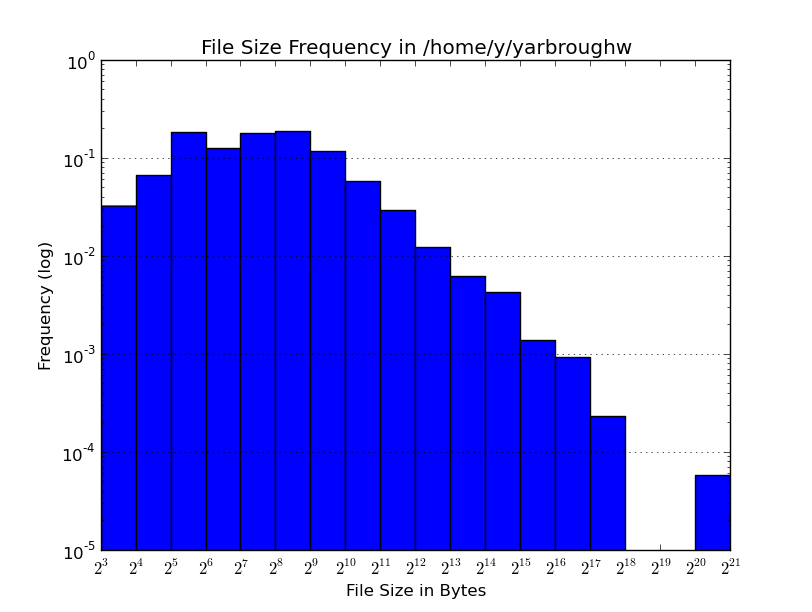
\includegraphics[scale=0.7]{assets/pycard-graph-1.png}

\newpage

\begin{lstlisting}
> $ python pycard.py ~/2013Fall
traversing file system with /home/y/yarbroughw/2013Fall as root...
traversing the file system took 29.728 ms.
analyzing results...
traversal from /home/y/yarbroughw/2013Fall shows:
   total file count 	=  49
   total size 		=  59289584 bytes (56.54 MB)
   average size 	=  1209991 bytes (1.15 MB)
   max file size 	=  21298031 bytes (20.31 MB)
   min file size 	=  590 bytes (0.00 MB)
   max depth 		=  7 directories
generating graph...
\end{lstlisting}

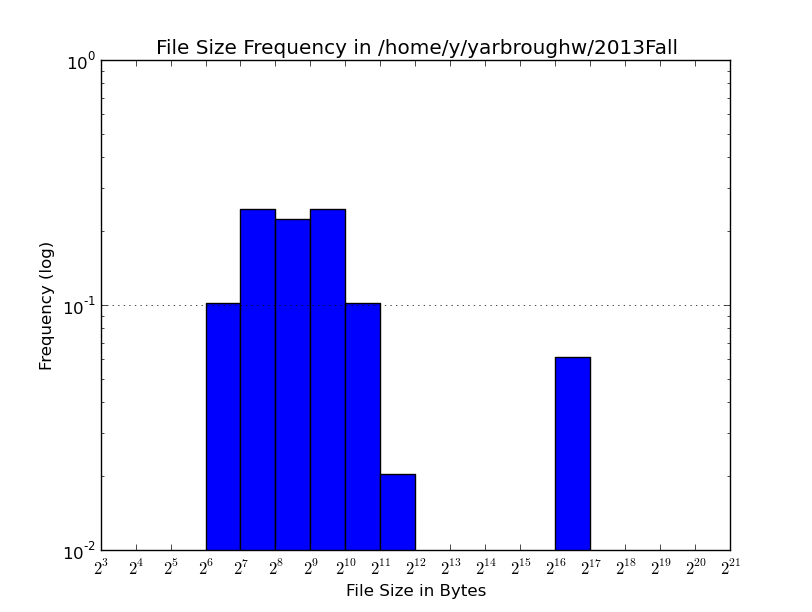
\includegraphics[scale=0.7]{assets/pycard-graph-2.png}

\newpage

\begin{lstlisting}
> $ python pycard.py ~/Downloads
traversing file system with /home/y/yarbroughw/Downloads as root...
traversing the file system took 225.403 ms.
analyzing results...
traversal from /home/y/yarbroughw/Downloads shows:
   total file count 	=  547
   total size 		=  22507340 bytes (21.46 MB)
   average size 	=  41146 bytes (0.04 MB)
   max file size 	=  9961287 bytes (9.50 MB)
   min file size 	=  8 bytes (0.00 MB)
   max depth 		=  10 directories
generating graph...
\end{lstlisting}

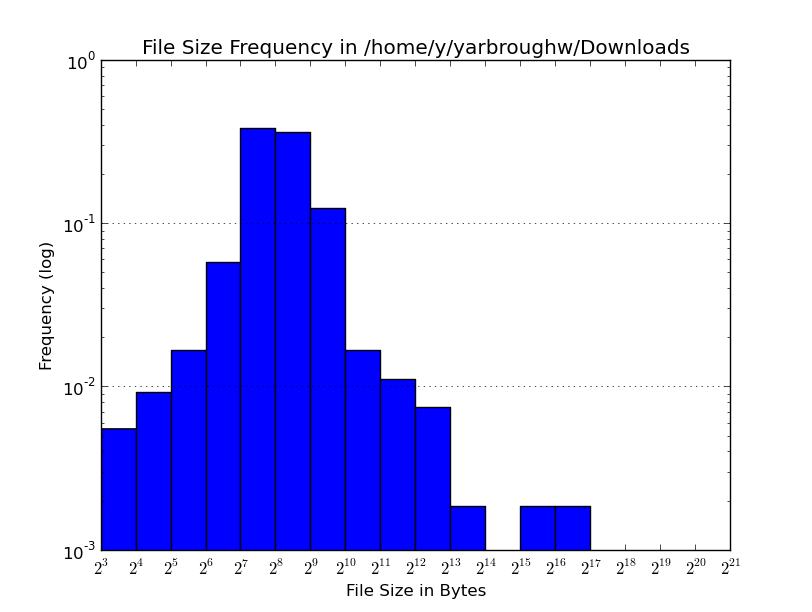
\includegraphics[scale=0.7]{assets/pycard-graph-3.png}

\newpage

\begin{lstlisting}
> $ python pycard.py ~/Misc/   
traversing file system with /home/y/yarbroughw/Misc as root...
traversing the file system took 350.295 ms.
analyzing results...
traversal from /home/y/yarbroughw/Misc shows:
   total file count 	=  521
   total size 		=  13548668 bytes (12.92 MB)
   average size 	=  26005 bytes (0.02 MB)
   max file size 	=  3498423 bytes (3.34 MB)
   min file size 	=  0 bytes (0.00 MB)
   max depth 		=  13 directories
generating graph...
                         
\end{lstlisting}

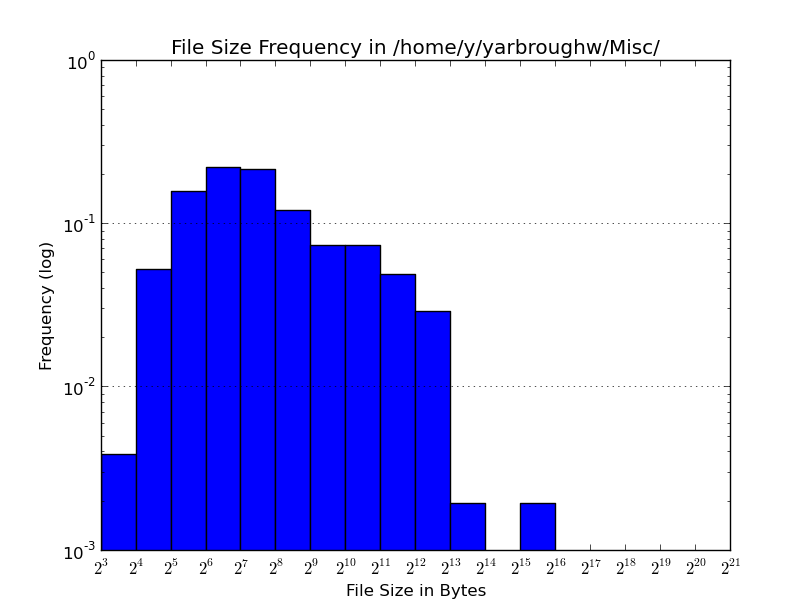
\includegraphics[scale=0.7]{assets/pycard-graph-4.png}

\newpage

\begin{lstlisting}
> $ python pycard.py ~/2014Spring/cs440/lab2/ 
traversing file system with /home/y/yarbroughw/2014Spring/cs440/lab2 as root...
traversing the file system took 75.915 ms.
analyzing results...
traversal from /home/y/yarbroughw/2014Spring/cs440/lab2 shows:
   total file count 	=  76
   total size 		=  387019 bytes (0.37 MB)
   average size 	=  5092 bytes (0.00 MB)
   max file size 	=  114277 bytes (0.11 MB)
   min file size 	=  15 bytes (0.00 MB)
   max depth 		=  12 directories
generating graph...
\end{lstlisting}

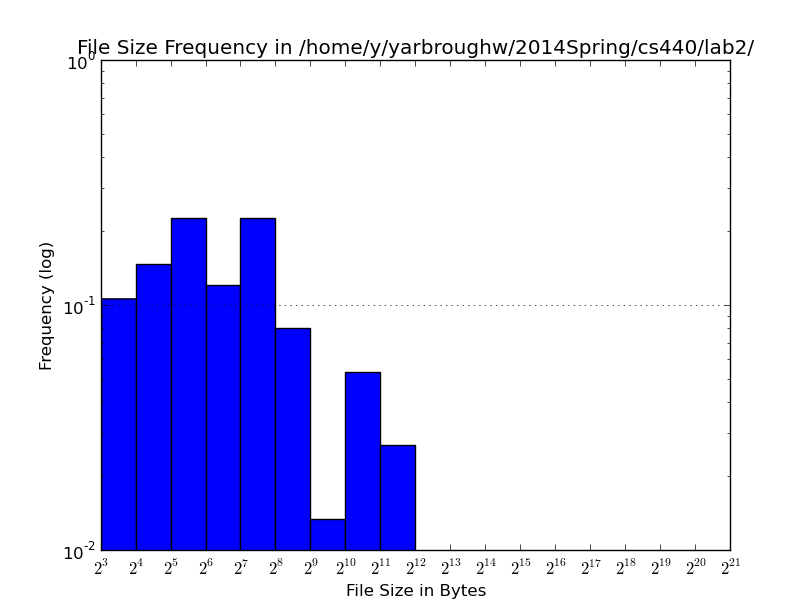
\includegraphics[scale=0.7]{assets/pycard-graph-5.png}

\newpage

\section{Experimental Study}

\end{document}
